%%%%%%%%%%%%%%%%%%%%%%%%%%%%%%%%%%%%%%%%%%%%%%%%%%%%%%%%%%%%%%%%%%%%%%%%%%%%%%%%
%2345678901234567890123456789012345678901234567890123456789012345678901234567890
%        1         2         3         4         5         6         7         8

\documentclass[letterpaper, 10 pt, conference]{ieeeconf}  % Comment this line out if you need  a4paper

%\documentclass[a4paper, 10pt, conference]{ieeeconf}      % Use this line for a4 paper

\IEEEoverridecommandlockouts                              % This command is only needed if
                                                          % you want to use the \thanks command

\overrideIEEEmargins                                      % Needed to meet printer requirements.

% See the \addtolength command later in the file to balance the column lengths
% on the last page of the document

% The following packages can be found on http:\\www.ctan.org
%\usepackage{graphics} % for pdf, bitmapped graphics files
\usepackage{graphicx}
%\usepackage{epsfig} % for postscript graphics files
%\usepackage{mathptmx} % assumes new font selection scheme installed
%\usepackage{times} % assumes new font selection scheme installed
%\usepackage{amsmath} % assumes amsmath package installed
%\usepackage{amssymb}  % assumes amsmath package installed

\title{\LARGE \bf
Software Architecture for Validation and Verification of Cooperative Autonomy of Multiple
Thermaling Gliders*
}

\author{Dmitrij Koniajev$^{1}$, Vladimir Fedorov$^{2}$ \\
    Nahum Camacho$^{3}$, Vladimir Dobrokhodov$^{4}$, and Kevin Jones$^{5}$% <-this % stops a space
\thanks{*The project has been supported over the last 3 years by a number of
sponsors including the NPS Consortium for Robotics and Unmanned Systems
Education and Research, the Army Research Lab, and "The Multidisciplinary
Studies Support for USMC Expeditionary Energy Office" program.}% <-this % stops a space
\thanks{$^{1}$Senior developer in the Demand-Side Platform team,
        Adform Lithuania, J. Jasinskio 16C, LT-01112 Vilnius, Lithuania,
        {\tt\small {dimchansky@gmail.com}}}%
\thanks{$^{2}$Postdoctoral researcher at the Department of Wind Energy,
        Technical University of Denmark, Building 114, Frederiksborgvej 399, DK-4000 Roskilde, Denmark
        {\tt\small {vlfe@dtu.dk}}}%
\thanks{$^{3-5}$authors are with the Department of Mechanical and Aerospace Engineering,
        Naval Postgraduate School, Monterey, CA 93943, USA
        {\tt\small {ncamacho, vldobr, jones}@nps.edu}}%
} % end of author

\begin{document}

\maketitle
\thispagestyle{empty}
\pagestyle{empty}


%%%%%%%%%%%%%%%%%%%%%%%%%%%%%%%%%%%%%%%%%%%%%%%%%%%%%%%%%%%%%%%%%%%%%%%%%%%%%%%%
\begin{abstract}
This paper describes the evolutionary steps in the design of cooperative
control capability of multiple autonomous soaring gliders. The paper
reviews the principal components necessary to enable the ''eternal`` flight
of a fleet of gliders, and presents initial comparison of simulated and
actual flight test results that demonstrate high-potential of collaborative
autonomous soaring. The paper primarily focuses on the design of the
software architecture that allows to verify the designed control algorithms
in a high-fidelity simulation prior to the actual flight. The software
architecture is based on the tight integration of Condor soaring flight
simulator with the advanced capabilities of MatLab/Simulink design
environment. The key benefits of the software for the flight control system
design include the ability to realistically represent the atmospheric
convective airflow and its interaction with 3D terrain, the high-fidelity
flight dynamics of a variety of soaring gliders, and the advance MathWorks'
tools of the control development and flight data analysis. The cooperative
capability is implemented by communicating the states of multiple gliders
over the network. Ultimately, the developed system allows verification and
validation of advanced cooperative control strategies and their comparison
against best practices of human piloted soaring flight.
\end{abstract}


%%%%%%%%%%%%%%%%%%%%%%%%%%%%%%%%%%%%%%%%%%%%%%%%%%%%%%%%%%%%%%%%%%%%%%%%%%%%%%%%
\section{INTRODUCTION}

Imagine a large team of gracefully soaring autonomous gliders, instrumented
with sensors capable of detecting convective air currents in the environment.
The gliders are launched from a remote location and assigned to provide, for
example, wide area network coverage or to serve as pseudo Low-Earth-Orbit
satellites to aid in fighting forest fires or to support border protection.
The gliders reach the area of operation and remain there unattended for an
extended period of time, perhaps up to a year. When a need for maintenance
arises the distributed intelligent algorithm reconfigures the team of gliders
and calls back the aircraft in need of service. In turn, when a substitute or
serviced aircraft returns, the same algorithm reconfigures the team to accept
the new player. Members of the flock can either operate in a distributed
fashion or fly together in a suitable formation to provide a more focused
capability. The latter may include cooperative distributed sensing to achieve
a desired sensor resolution, tracking of weather formations, border patrol,
and many other tasks that are currently provided by much larger, heavier, and
more expensive systems.

There have been several projects that have sought to capitalize on convective
lift in the environment to offset or remove the need for propulsion. First
demonstrated by human pilots in 1900s (see \cite{Simons:1998}) the idea of
soaring in convective air became feasible for onboard autonomous
implementation only in the 1990s, see \cite{Wharington:1998}. A challenge for
these vehicles revolves around locating the regions of advantageous lift.
While enabling the desired functionality by primarily mimicking the birds
flight and indeed achieving significant extended flight capabilities (see
\cite{Edwards:2008}, \cite{Allen:2006}, and \cite{Allen:2007}), most of the
algorithms used heuristics in the identification of the updraft strength, its
potential utility in energy gain, and the decision of when and how to enter
the updraft. The reason for employing heuristic approaches is obvious, since
both the strength of the updraft and its efficiency are both subject to
significant uncertainties and are hard to formalize. The most recent
development by~\cite{AKlass_CDC:2012,AKlass_JGCD:2012} demonstrated that
teaming aircraft working cooperatively could improve the probability of
successful detection and exploitation of thermals by splitting up the search
task and sharing location data for regions of lift. Combining the ability to
exploit natural lift in the environment with photo-voltaic or wind-driven
energy production, the vehicles should be able to stay aloft $24/7$, while
still having enough additional energy to support the weight and power of
meaningful payloads.


\section{Integrated Control Development Environment}

\subsection{Concept of Operation}
In order to enable the collaborative flight of autonomous thermal soaring
gliders it is envisioned that each glider is equipped with online algorithms
of convective thermals search, detection, and exploitation, as well as the
collaborative decision making and communication methods; see the concept in
Figure.\ref{fig:coop_scheme}.
%%%%%%%%%%
\begin{figure}[thpb]
  \centering
  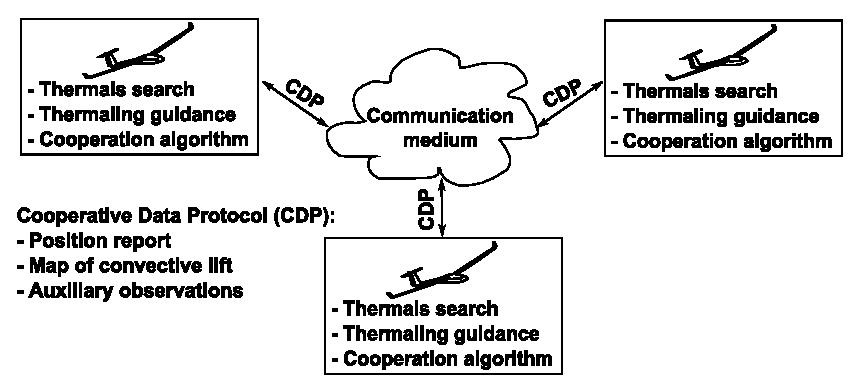
\includegraphics[scale=0.6]{Figures/coop_scheme_small.eps}
  \caption{Cooperation of autonomous gliders.}
  \label{fig:coop_scheme}
\end{figure}
%%%%%%%%%%
The algorithms will run online to identify the inherent flight dynamics of the
glider which are used to detect the thermal updrafts. When flying in the
updraft, the thermaling guidance algorithm is engaged to enable the maximum
energy harvesting efficiency of the updraft’s free energy, and on the other
hand estimates the updraft geometry and motion, that are used to georeference
the updraft and share its utility properties (strength) across the network of
collaborative gliders. Finally, the distributed knowledge about the existing
updrafts needs to be intelligently utilized to maximize the benefit of team
of gliders flying with a specific operational objective.

\subsection{Software Architecture of High-fidelity Control Design Environment}
To verify the efficiency of the developed algorithms a number of flight tests
needs to be performed. While recognizing the value of flight testing, and
still accounting for the complexity of flight experimentation, the project
builds a high-fidelity numerical simulation and control design environment
that provides the convenience and rigor of control algorithm development. To
this end the project developed a realistic simulation environment that is
based on tight integration of MatLab/Simulink \cite{MATLAB:2013} control
design capabilities with the high-fidelity flight dynamics and atmospheric
effects of the Condor soaring simulator, see \cite{Condor:2013:Online}.

%Besides providing a wide nomenclature of gliders, the software integrates the
%cooperative behaviors of multiple agents that is essential to the project;
%the collaboration is enabled by sharing the states of gliders over the
%network.

The Condor soaring simulator is one of the most realistic simulators compared
to real life soaring; the software has been designed focusing on the
fundamental principles of aerodynamic flight, and atmosphere and weather
physics. Recognized for the high fidelity of simulating of the fundamental
principals of soaring flight and the high realism of visualization, this
simulator has been used by human glider pilots to acquire initial skills and
to maintain their proficiency during off-season. The Condor allows to advance
piloting skills in different wing loading conditions and weight balancing,
various flight regimes including stall and spin, and even to test pilots
ability to recover the damaged aircraft. Furthermore, the pilots can
experience soaring flight in different areas of the world, test their skills
against other pilots in individual and team competitions. The key features of
the Condor soaring simulator that are important enablers of the autonomous
soaring are provided below, see \cite{Condor:2013:Online} for more details:
\begin{itemize}
  \item advanced 6DOF flight dynamics model run by real-time high-fidelity
      physics engine (up to 500 cycles per second);
  \item accurate sailplane performance and handling qualities including the
      flight at critical and beyond critical angles of attack;
  \item sailplane's damage simulation including the flutter, high $g$
      stress, and aircraft collisions;
  \item realistic representation of the thermals life cycle that starts
      from the ground and expands up to the cloud base; the cloud grows
      bigger and more dense and later dissipates thus causing the air below
      it to sink;
  \item the location and strength of thermals is based on the exposure of
      terrain to sun and accounts for the ground features like forests,
      swamps, fields, and man-made structures like cities and villages;
  \item realistic daily sun travel which affects the frequency and strength
      of thermals;
  \item models up-slope wind on sunny ridges (anabatic winds);
  \item models ridge lift with leeward downwind and turbulence, venturi
      effects;
  \item models waves behind ridges; wavelength depends on wind speed and
      stability of the atmosphere;
  \item defines correct atmospheric pressure, density and temperature
      versus height;
  \item implements $3D$ isotropic turbulence model for thermal convection
      and mechanical turbulence.
\end{itemize}
%%%%%%%%%%
\begin{figure}[thpb]
  \centering
  \includegraphics[scale=0.4]{Figures/api_arch.eps}
  \caption{The Condor API.}
  \label{fig:api_arch}
\end{figure}
%%%%%%%%%%

In order to harness the features of high-fidelity soaring simulation and
connect them with advanced capabilities of control systems design provided by
MatLab/Simulink, an unobtrusive and invisible for the original Condor
software service has been developed. The key objective for this ``Condor
API'' service is to provide low-level communication between Simulink and
Condor. Presented in Figure.\ref{fig:api_arch} the Condor API service
significantly extends the aircraft data which Condor simulator streams to
external applications. The extended data set includes data like the plane
position, true airspeed, wind course, wind speed, MacCready setting (MC),
control surfaces (ailerons, elevator, rudder and air-break) deflection. The
Condor API then streams the extended aircraft data to an external application
(MatLab/Simulink) using UDP protocol. Utilizing Condor API, an external
application then can send the control surface commands back to the Condor API
service via UDP, thus effectively establishing the software in the loop (SIL)
environment, see Figure.\ref{fig:SIL}.
%%%%%%%%%%
\begin{figure}[thpb]
  \centering
  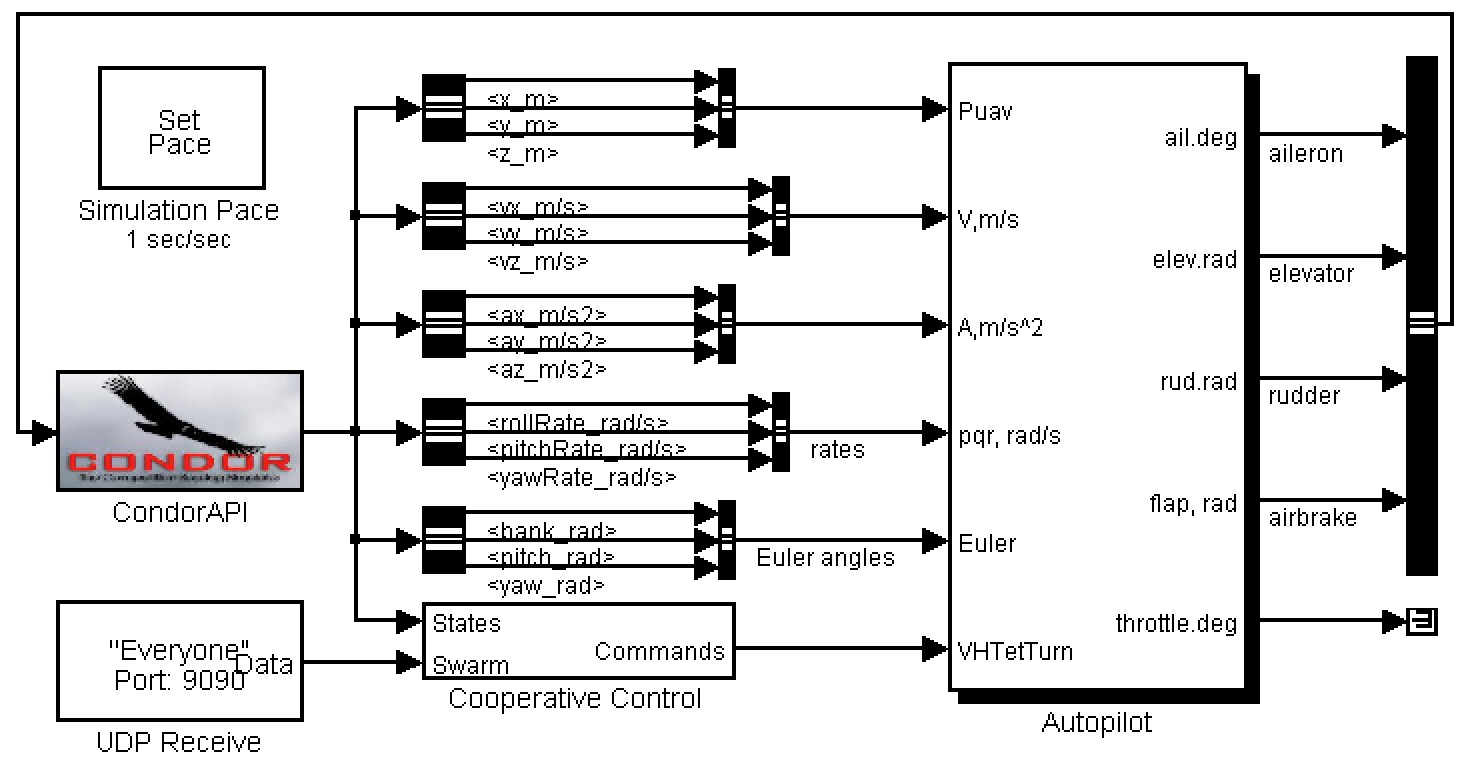
\includegraphics[scale=0.3]{Figures/SIL.eps}
  \caption{Integration of Simulink and Condor capabilities.}
  \label{fig:SIL}
\end{figure}
%%%%%%%%%%

Harnessing the features of Condor soaring simulator allows leveraging the
advanced capabilities of the MatLab/Simulink control design environment, thus
resulting in a high-fidelity control design setup for cooperative soaring
flight. Thus, the developed setup provides a convenient interface for the
researchers that allows them to quickly connect to the simulator and focus on
the novel algorithm development.

\subsection{Potential Capabilities and Future Improvements}

In the current implementation the intelligent agents, which are implemented
by the Simulink model, share the states of a glider and its local onboard
knowledge of thermaling convective lift via multicast UDP messages. This
communication mechanism allows to run the Condor soaring simulator and
Matlab/Simulink on different machines connected over the local network.
Moreover, this capability enables a competitive flight of multiple soaring
gliders inside one local network.

At the same time the UDP communication has also its flaws. Since the UDP
multicast over the Internet is not possible in general because the multicast
packages are not routed, the cooperative competitive flight of multiple
autonomous gliders with human pilots over Internet is not possible. Another
limitation is that multiple groups of autonomous agents located on the same
local network at the same time will interfere with each other.

The future version of the Condor API service could be improved by building
distributed Condor API system, which would consist of a number of Condor API
services communicating with each other. The distribution mechanism could be
implemented using TCP/IP sockets like in the distributed Erlang systems
(\cite{Erlang:2013:Online}) or Akka actors (\cite{Akka:2013:Online}). This
will solve the aforementioned problems and allow to create more powerful
distributed agents.

Verification and validation of cooperative control strategies that take
significant time to evolve in a distributed settings can be very difficult.
To facilitate early identification of correct strategies and save time a
visualization of cooperative strategies might be very effective. To this end,
the Condor API service has been expanded with ``FlightRadar'' external
application that provides the capability to represent multiple evolving
trajectories in one $3D$ map. The

To visualize the strategies of multiple competing soaring gliders in
real-time the FlightRadar streams information to Google
Maps~\cite{GoogleMaps:2013:Online}, see an example of a half hour flight in
Figure.\ref{fig:FlightRadar}.
%%%%%%%%%%
\begin{figure}[thpb]
  \centering
  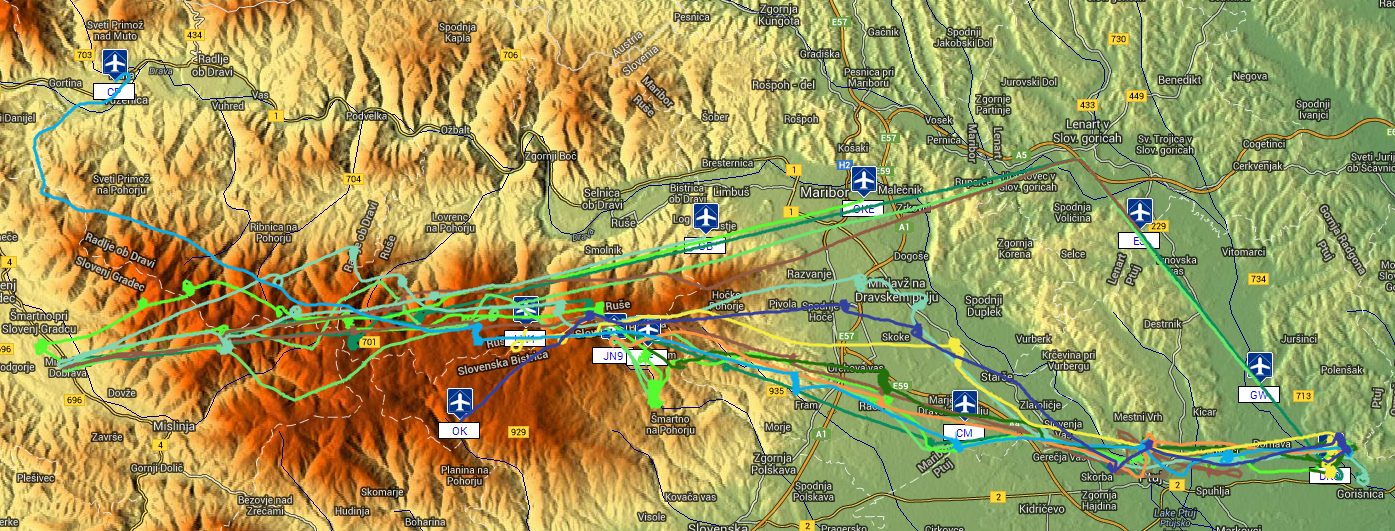
\includegraphics[scale=0.17]{Figures/flightradar_highlevel.eps}
  \caption{Evolution of cooperative strategies.}
  \label{fig:FlightRadar}
\end{figure}
%%%%%%%%%%

\section{Principles of Convective Lift Detection and Cooperative Exploitation}
...

\subsection{ Thermals Detection and Exploitation by Single Glider}

Sink polar

Total Energy approach

Guidance of a single glider

\subsection{ Cooperative Strategies}

....

\section{Experimental Results}

Present results of 3 gliders searching for a single thermal in a bounded box.
One of them finds the thermal, estimates its position and shares knowledge
with the rest of the team. The other 2 gliders come to the same spot and
start climbing.

As an illustration of the achieved capabilities,
Figure.\ref{fig:CoopFlightPaths} represents the cooperative flight of three
gliders in a simplified scenario introduced above. The gliders start their
flight simultaneously at the same altitude, and initially spend some time in
search for thermals. When glider $\#1$ detects an updraft utilizing either of
the thermal detection approaches, and shares the information about the
thermal, the other two gliders arrive to the same thermal and successfully
gain height all together. Time history of the altitude of three cooperative
gliders is presented next in Figure.\ref{fig:CoopFlightHeight}. The result
clearly demonstrates the benefits and significant potential of collaborative
strategies in harvesting the convective updraft energy from the environment.
%%%%%%%%%%
\begin{figure}[thpb]
  \centering
  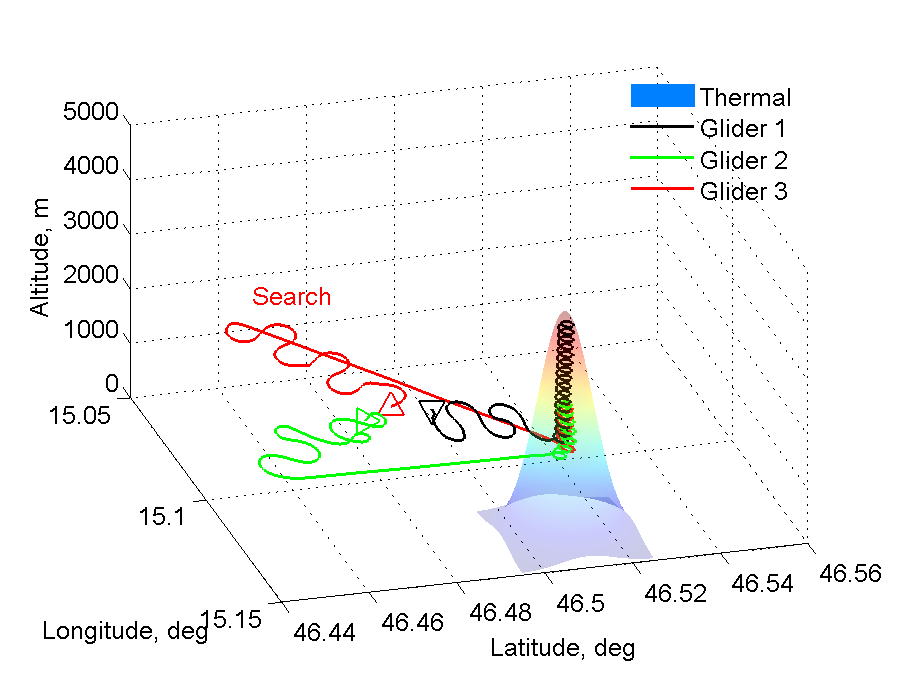
\includegraphics[scale=0.41]{Figures/paths_cooperative_flight.eps}
  \caption{Cooperative flight of three gliders; starting at different locations
  they all converge to the same updraft when glider $\#1$ finds it and
  shares its estimated location.}
  \label{fig:CoopFlightPaths}
\end{figure}
%%%%%%%%%%
%%%%%%%%%%
\begin{figure}[thpb]
  \centering
  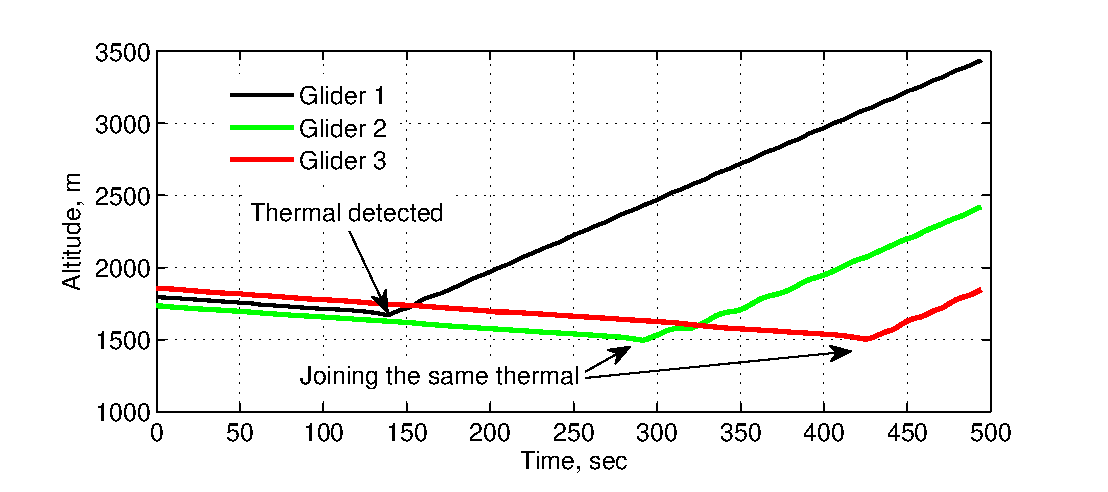
\includegraphics[scale=0.39]{Figures/Coop_gain_altitude.eps}
  \caption{An example of cooperative flight of three gliders.}
  \label{fig:CoopFlightHeight}
\end{figure}

%%%%%%%%%%%%%%%%%%%%%%%%%%%%%%%%%%%%%%%%%%%%%%%%%%%%%%%%%%%%%%%%%%%%%%%%%%%%%%%%
\section*{APPENDIX}

Appendixes can be used to show the snippets of configuration files.

\section*{ACKNOWLEDGMENT}
The project has been supported over the last 3 years by a number of sponsors
including the NPS Consortium for Robotics and Unmanned Systems Education and
Research, the Army Research Lab, and "The Multidisciplinary Studies Support
for USMC Expeditionary Energy Office" program. The authors would like to
mention the contribution of graduate students Andrew Streenan and Joshua
Weiss for providing results of their final project and contributing to the
extensive simulation research.

%%%%%%%%%%%%%%%%%%%%%%%%%%%%%%%%%%%%%%%%%%%%%%%%%%%%%%%%%%%%%%%%%%%%%%%%%%%%%%%%

\bibliographystyle{IEEEtran}
\bibliography{IEEEabrv,iros}



\end{document}
